\documentclass{article}
\usepackage[utf8]{inputenc}

\title{Written Assignment 2}
\author{Benny Chen}
\date{\today}

\usepackage{color}
\usepackage{amsthm}
\usepackage{amssymb} 
\usepackage{amsmath}
\usepackage{listings}
\usepackage{xcolor}
\usepackage{listings}
\usepackage{graphicx}
\usepackage{pgfplots}
\usepackage{tikz}
\usepackage{enumitem}
\usepackage[hidelinks]{hyperref}

\definecolor{codegreen}{rgb}{0,0.6,0}
\definecolor{codegray}{rgb}{0.5,0.5,0.5}
\definecolor{codepurple}{rgb}{0.58,0,0.82}
\definecolor{backcolour}{rgb}{0.95,0.95,0.92}

\lstdefinestyle{mystyle}{
    backgroundcolor=\color{backcolour},   
    commentstyle=\color{codegreen},
    keywordstyle=\color{magenta},
    numberstyle=\tiny\color{codegray},
    stringstyle=\color{codepurple},
    basicstyle=\ttfamily\footnotesize,
    breakatwhitespace=false,         
    breaklines=true,                 
    captionpos=b,                    
    keepspaces=true,                 
    numbers=left,                    
    numbersep=5pt,                  
    showspaces=false,                
    showstringspaces=false,
    showtabs=false,                  
    tabsize=2
}

\lstset{style=mystyle}

\begin{document}

\maketitle

\section{DBSCAN}

Suppose we apply DBScan algorithm with Eps = 0.15 (in Euclidean distance) and MinPts = 3.

\begin{center}
    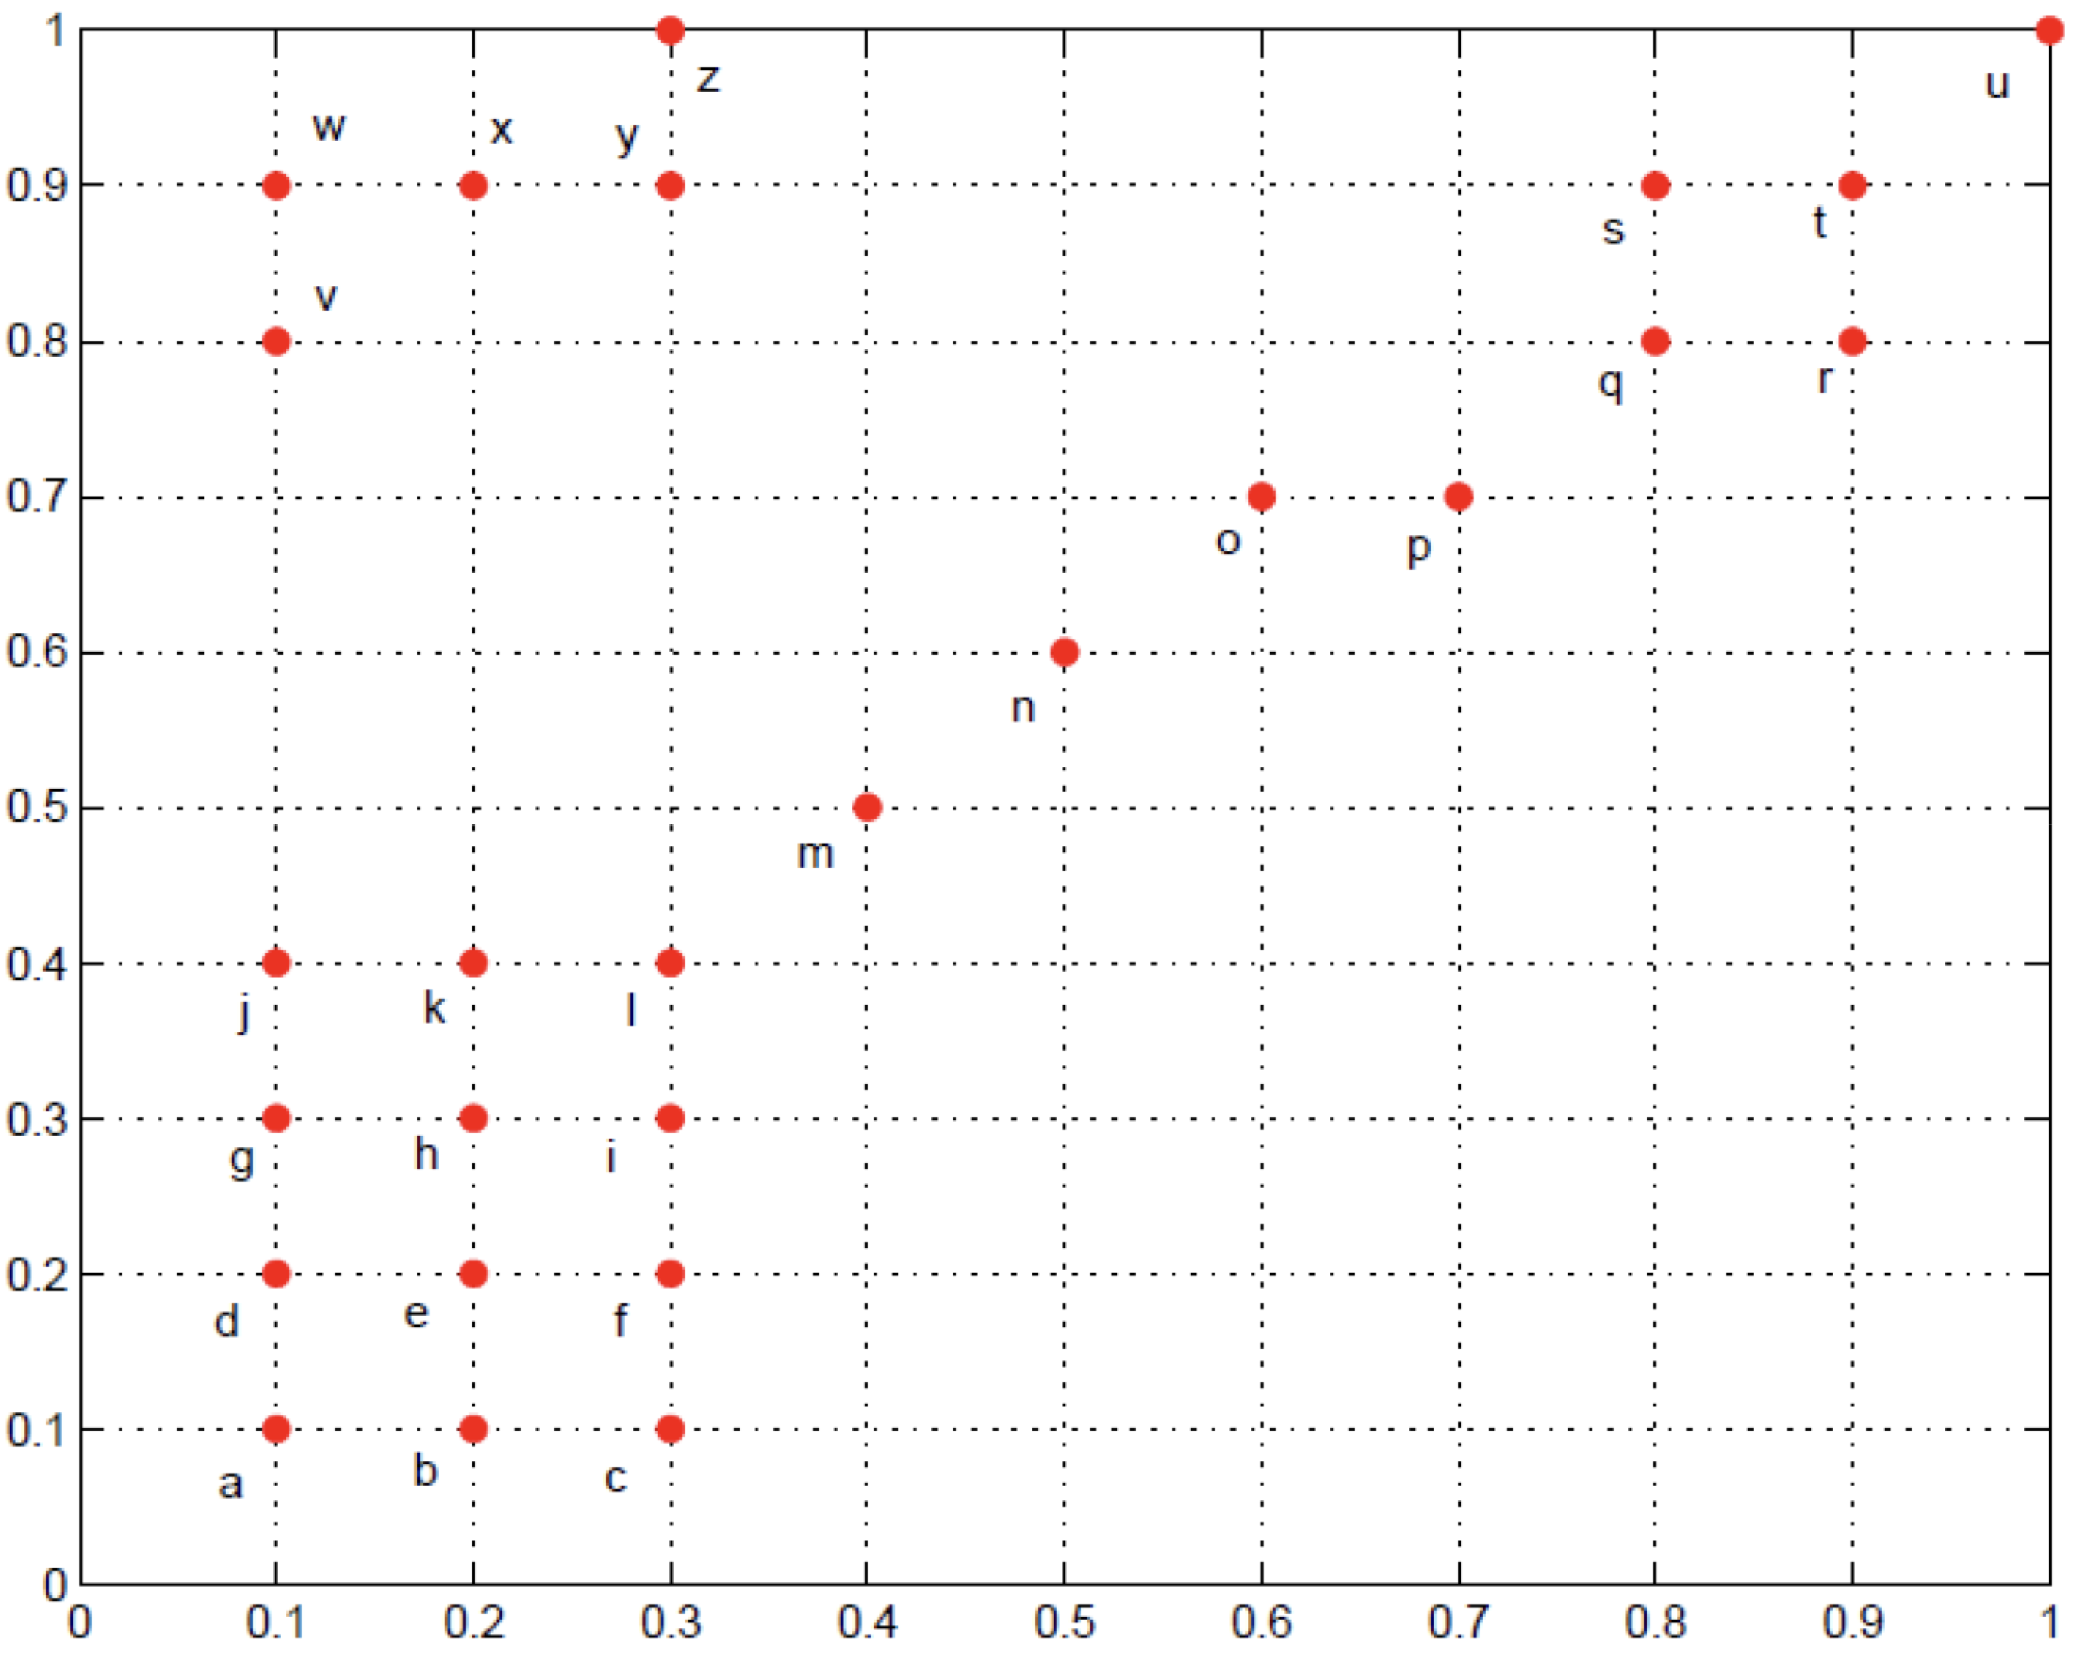
\includegraphics[width=\textwidth]{./images/Q1image.png}
\end{center}  

\begin{enumerate}[label=(\alph*)]
    \item List all the core points in the diagram (you can use the labels of the data points in the diagram). \textit{Note: a point is considered a core point if there are \textbf{more than Min Pts} number of points \textbf{(including the point itself)} within a neighborhood of radius Eps.}
    \item List all the border points in the diagram.
    \item List all the noise points in the diagram.
    \item Using the DBScan algorithm, how many clusters will be obtained from the data set?
\end{enumerate}

\begin{enumerate}[label=(\alph*)]
    \item Given the graph, we can see the core points of any point that as at least 3 other points in the neighborhood of radius 0.15. The core points are: $A, B, C, D, E, F, G, H, I, J, K, L, Q, R, S, T, X$.
    \item Given the graph, we can see the border points of any point that has less than 3 other points in the neighborhood of radius 0.15. The border points are: $M, P, U, V, W, Y, Z$.
    \item Given the graph, we can see the noise points of any point that is neither a core point nor a border point. The noise points are: $N, O$.
    \item After finding all core, border, and noise points, we can now go through each core point and cluster them up. By doing this we get a total of 3 clusters.
\end{enumerate}

\section{Dimensionality Reduction}

Consider the following matrix, representing four sample points $X \in R^2$
\begin{equation*}
    X = \begin{bmatrix}
        4 & 1 \\
        2 & 3 \\
        5 & 4 \\
        1 & 0
    \end{bmatrix}
\end{equation*}

\noindent
(a) We want to represent the data in only one dimension, so we turn to PCA. Please compute the \textit{unit-length} principal component directions of X (unit length means that the resulting vector's norm should be equal to 1, \textit{e.g}., you should return a vector $(a, b)$ that has $a^2 + b^2 = 1$).
\\
(Suggested steps: center the data, calculate the sample covariance matrix, calculate the eigenvectors and eigenvalues, identify the principal component, please provide the calculation process).
\\
Note: sample covariance matrix is based on:
\begin{equation*}
    cov_{x,y} = \frac{\Sigma(x_i - \bar{x})(y_i - \bar{y})}{N-1}
\end{equation*}
\\
We first compute the mean per dimension then subtract the mean from each value to center it which we get:
[4, 2, 5, 1] = 3 and [1, 3, 4, 0] = 2
\begin{equation*}
    X = \begin{bmatrix}
        1 & -1 \\
        -1 & 1 \\
        2 & 2 \\
        -2 & -2
    \end{bmatrix}
\end{equation*}
We then find the covariance matrix using the above equation which we get:
\begin{equation*}
    cov_{x,y} = \frac{(1*-1+-1*1+2*2+-2*-2)}{4-1} = 2
\end{equation*}
\begin{equation*}
    c_x = \frac{1^2 + -1^2 + 2^2 + -2^2}{4-1} = \frac{10}{3}
\end{equation*}
\begin{equation*}
    c_y = \frac{-1^2 + 1^2 + 2^2 + -2^2}{4-1} = \frac{10}{3}
\end{equation*}

\begin{equation*}
    \begin{bmatrix}
        \frac{10}{3} & 2 \\
        2 & \frac{10}{3}
    \end{bmatrix}
\end{equation*}

We then find the eigenvalues and eigenvectors of the covariance matrix which we get:
\begin{equation*}
    det(
    \begin{bmatrix}
        \frac{10}{3} & 2 \\
        2 & \frac{10}{3}
    \end{bmatrix}
    - \lambda
    \begin{bmatrix}
        1 & 0 \\
        0 & 1
    \end{bmatrix}
    )
\end{equation*}
\begin{equation*}
    \begin{bmatrix}
        \frac{10}{3} - \lambda & 2 \\
        2 & \frac{10}{3} - \lambda
    \end{bmatrix} = 0
\end{equation*}
\begin{equation*}
    \lambda^2 - \frac{20\lambda}{3} + \frac{64}{9} = 0
    = \begin{bmatrix}
        \frac{16}{3} \\
        \frac{4}{3}
    \end{bmatrix}
\end{equation*}
Along with eigenvectors:
\begin{equation*}
    v_1 = 
    \begin{bmatrix}
        0.70710678 \\
        0.70710678 
    \end{bmatrix}
    v_2 =
    \begin{bmatrix}
        - 0.70710678 \\
        0.70710678 
    \end{bmatrix}
\end{equation*}
0.70710678 and -0.70710678 squared are both .5 resulting in a unit length vector of 1 for both. The principal component is the eigenvector with the largest eigenvalue which is $v_1$.
\\
(b) Given the following 3D input data, $X \in R^3$, \textit{i.e,}
\begin{equation*}
    X = \begin{bmatrix}
        1 & 1 & 9 \\
        2 & 4 & 6 \\
        3 & 7 & 4 \\
        4 & 11 & 4 \\
        5 & 9 & 2
    \end{bmatrix}
\end{equation*}

\noindent
Please compute the \textit{unit-length} principal component \textit{which corresponds to the largest eigenvalue.}
\\
(Suggested steps: center the data, calculate the sample covariance matrix, calculate the eigenvectors and eigenvalues, identify the principal component, please provide the calculation process).
\\\\
We again compute the mean per dimension then subtract the mean from each value to center it which we get:
[1, 2, 3, 4, 5] = 3 and [1, 4, 7, 11, 9] = 6.4 and [9, 6, 4, 4, 2] = 5

\begin{equation*}
    X = \begin{bmatrix}
        -2  & -5.4  & 4 \\
        -1  & -2.4  & 1 \\
        0   & 0.6   & -1 \\
        1   & 4.6   & -1 \\
        2   & 2.6   & -3
    \end{bmatrix}
\end{equation*}

We then find the covariance matrix using the above equation which we get:

\begin{equation*}
    c_x = \frac{(-2)^2+(1)^2+(0)^2+(1)^2+(2)^2}{4} = 2.5
\end{equation*}
\begin{equation*}
    c_y = \frac{(-5.4)^2+(-2.4)^2+(0.6)^2+(4.6)^2+(2.6)^2}{4} = 15.8
\end{equation*}
\begin{equation*}
    c_z = \frac{(4)^2+(1)^2+(-1)^2+(-1)^2+(-3)^2}{4} = 7
\end{equation*}
\begin{equation*}
    cov_{x,y} = \frac{(-2 * -5.4 + -1 * -2.4 + 0 * 0.6 + 1 * 4.6 + 2 * 2.6)}{4} = 5.75
\end{equation*}
\begin{equation*}
    cov_{x,z} = \frac{(-2 * 4 + -1 * 1 + 0 * -1 + 1 * -1 + 2 * -3)}{4} = -4
\end{equation*}
\begin{equation*}
    cov_{y,z} = \frac{(-5.4 * 4 + -2.4 * 1 + 0.6 * -1 + 4.6 * -1 + 2.6 * -3)}{4} = -9.25
\end{equation*}

Which we then get the covariance matrix:
\begin{equation*}
    \begin{bmatrix}
        2.5 & 5.75 & -4 \\
        5.75 & 15.8 & -9.25 \\
        -4 & -9.25 & 7
    \end{bmatrix}
\end{equation*}

We then find the eigenvalues and eigenvectors of the covariance matrix which we get:

\begin{equation*}
    det(\begin{bmatrix}
        2.5 & 5.75 & -4 \\
        5.75 & 15.8 & -9.25 \\
        -4 & -9.25 & 7
    \end{bmatrix}) - \lambda
    \begin{bmatrix}
        1 & 0 & 0 \\
        0 & 1 & 0 \\
        0 & 0 & 1
    \end{bmatrix} = 0
\end{equation*}
\begin{equation*}
    \begin{bmatrix}
        2.5 - \lambda & 5.75 & -4 \\
        5.75 & 15.8 - \lambda & -9.25 \\
        -4 & -9.25 & 7 - \lambda
    \end{bmatrix} = 0
\end{equation*}
\begin{equation*}
    -\lambda^3 + \frac{253\lambda^2}{10} - \frac{1319\lambda}{40} + \frac{617}{160} = 0 = \begin{bmatrix}
        23.9287 \\
        0.129806 \\
        1.24151
    \end{bmatrix}
\end{equation*}

With eigenvalues of 23.9287, 0.129806, and 1.24151 and eigenvectors of:
\begin{equation*}
    v_1 = 
    \begin{bmatrix}
        0.3110472 \\
        0.801393 \\
        -0.511249
    \end{bmatrix}
    v_2 =
    \begin{bmatrix}
        0.913843 \\
        -0.10335 \\
        0.392643
    \end{bmatrix}
    v_3 =
    \begin{bmatrix}
        -0.261722 \\
        0.589106 \\
        0.74497
    \end{bmatrix}
\end{equation*}

The principal component is the eigenvector corresponding to the largest eigenvalue which is:
\begin{equation*}
    v_1 = 
    \begin{bmatrix}
        0.3110472 \\
        0.801393 \\
        -0.511249
    \end{bmatrix}
\end{equation*}
With a variance of 23.9287.


\section{Web Data Mining}

(a) Given the 4 web pages and their mutual links, find their \textbf{Page Ranks according to our lecture notes.} Suppose we initialize all ranks as 1.

\begin{enumerate}[label=(\roman*)]
    \item Please provide the convergence ranks based on r = Mr. Note that for the stochastic matrix, please use the alphabetical order (from A to D) to list the web pages in the matrix. You can write a program to calculate but you are not required to submit the program. You can show me at which iteration the rank starts to converge.
    \item Please provide the convergence ranks based on r = 0.9Mr + c, where $c = [0.1 0.1 0.1 0.1]^T$. You can write a program to calculate but you are not required to submit the program. You can show me at which iteration the rank starts to converge.
\end{enumerate}
\begin{enumerate}[label=(\alph*)]
    \item \begin{enumerate}[label=(\roman*)]
        \item Given the given 4 web pages, we can create a stochastic matrix as follows:
    \begin{table}[h]
        \begin{tabular}{lllll}
          & A       & B & C     & D \\
        A & 0       & 0 & 1     & 0 \\
        B & 0.5     & 0 & 0     & 0 \\
        C & 0.5     & 1 & 0     & 1 \\
        D & 0       & 0 & 0     & 0
        \end{tabular}
        \centering
    \end{table}
    \begin{equation*}
        M = \begin{bmatrix}
            0       & 0 & 1     & 0 \\
            0.5     & 0 & 0     & 0 \\
            0.5     & 1 & 0     & 1 \\
            0       & 0 & 0     & 0
        \end{bmatrix}
        r = M* \begin{bmatrix}
            1 \\
            1 \\
            1 \\
            1
        \end{bmatrix} = 
        \begin{bmatrix}
            1 \\
            0.5 \\
            2.5 \\
            0
        \end{bmatrix}
    \end{equation*}
    We can now do this iteratively using $r = Mr$ until the ranks converge to get the following ranks:
    \begin{equation*}
        r = \begin{bmatrix}
            1.60 \\
            0.80 \\
            1.60 \\
            0
        \end{bmatrix}
    \end{equation*}
    \item We can then calculate the rank of each page using the following formula:
    \begin{equation*}
        r = 0.9Mr + c
    \end{equation*}
    \begin{equation*}
        r = 0.9
        \begin{bmatrix}
            0       & 0 & 1     & 0 \\
            0.5     & 0 & 0     & 0 \\
            0.5     & 1 & 0     & 1 \\
            0       & 0 & 0     & 0
        \end{bmatrix}
        \begin{bmatrix}
            1 \\
            1 \\
            1 \\
            1
        \end{bmatrix}
        + \begin{bmatrix}
            0.1 \\
            0.1 \\
            0.1 \\
            0.1
        \end{bmatrix}
    \end{equation*}
    We can then calculate the rank of each page using $r = 0.9Mr + c$ iteratively until the ranks converge:
    \begin{equation*}
        r = \begin{bmatrix}
            0.9(0*1 + 0*1 + 1*1 + 0*1)\\
            0.9(0.5*1 + 0*1 + 0*1 + 0*1)\\
            0.9(0.5*1 + 1*1 + 0*1 + 1*1)\\
            0.9(0*1 + 0*1 + 0*1 + 0*1)
        \end{bmatrix}
        + \begin{bmatrix}
            0.1 \\
            0.1 \\
            0.1 \\
            0.1
        \end{bmatrix}
        = \begin{bmatrix}
            1 \\
            0.55 \\
            2.35 \\
            0.1
        \end{bmatrix}
    \end{equation*}
    We then get the following ranks:
    \begin{equation*}
        r = \begin{bmatrix}
            1.527 \\
            0.7872 \\
            1.585 \\
            0.1
        \end{bmatrix}
    \end{equation*}
    \end{enumerate}
    \item We first make a adjacency matrix of the given web pages:
    \begin{table}[h]
        \begin{tabular}{lllll}
          & A   & B & C     & D \\
        A & 0   & 1 & 1     & 0 \\
        B & 0   & 0 & 1     & 0 \\
        C & 1   & 0 & 0     & 0 \\
        D & 0   & 0 & 1     & 0
        \end{tabular}
        \centering
    \end{table}
    \\With the $M^T, MM^T, and M^TM$ as:
    \begin{equation*}
        M^T =
        \begin{bmatrix}
        0   & 0 & 1     & 0 \\
        1   & 0 & 0     & 0 \\
        1   & 1 & 0     & 1 \\
        0   & 0 & 0     & 0
        \end{bmatrix}
        MM^T =
        \begin{bmatrix}
        2   & 1 & 0     & 1 \\
        1   & 1 & 0     & 1 \\
        0   & 0 & 1     & 0 \\
        1   & 1 & 0     & 1
        \end{bmatrix}
        M^TM =
        \begin{bmatrix}
        1   & 0 & 0     & 0 \\
        0   & 1 & 1     & 0 \\
        0   & 1 & 3     & 0 \\
        0   & 0 & 0     & 0
        \end{bmatrix}
        \centering
    \end{equation*}
    We can now calculate the hub and authority scores, we first normalize $MM^T \& M^TM$ or Hub and Authority scores respectively:
    \begin{equation*}
        MM^T =
        \begin{bmatrix}
        \frac{4}{4 + 3 + 1 + 3} * 4 \\
        \frac{3}{4 + 3 + 1 + 3} * 4 \\
        \frac{1}{4 + 3 + 1 + 3} * 4 \\
        \frac{3}{4 + 3 + 1 + 3} * 4
        \end{bmatrix} =
        \begin{bmatrix}
        1.45 \\
        1.09 \\
        0.36 \\
        1.09
        \end{bmatrix}
        M^TM =
        \begin{bmatrix}
        \frac{1}{1 + 2 + 4 + 0} * 4 \\
        \frac{2}{1 + 2 + 4 + 0} * 4 \\
        \frac{4}{1 + 2 + 4 + 0} * 4 \\
        \frac{0}{1 + 2 + 4 + 0} * 4
        \end{bmatrix} =
        \begin{bmatrix}
            .57 \\
            1.14 \\
            2.28 \\
            0
        \end{bmatrix}
        \centering
    \end{equation*}
    We then do this iteratively until the scores converge:
    \begin{equation*}
        h = MM^T h = \begin{bmatrix}
            1.65 \\
            1.17 \\
            0 \\
            1.17
        \end{bmatrix}
        a = M^TM a = \begin{bmatrix}
            0 \\
            1.1715 \\
            2.828 \\
            0
        \end{bmatrix}
    \end{equation*}
\end{enumerate}

\section{SVM}

\begin{enumerate}[label=(\alph*)]
    \item Quick Questions on SVM Consider the following training points. Circles are classified as positive examples with label + 1 and triangles are classified as negative examples with label -1.
    \begin{enumerate}[label=(\roman*)]
        \item Which points are the support vectors? (You do not need to provide the derivation process)
        \item If we add the sample point × = [5, 1] with label -1 (triangle) to the training set, which points are the support vectors?
        \item Recall that an SVM has the form of $y_i(w^T * X_i + b) \ge 1$, where $y_i$'s are the labels and $X_i$'s are the training data points. What is the geometric relationship between the weight vector w and the decision boundary of SVM (if you draw them in the 2-D plane, how would they geometrically look like)?
    \end{enumerate}
    \item Model Derivation Consider the 2-dimensional data shown in the following figure. There are three data points, two of them are classified as positive (red circles) and one is negative (blue square). Let the decision boundary of the linear classifier be $w^Tx + b = 0$ (shown as a red line in the diagram).
    The geometric margin of each data point is the perpendicular distance between each data point to the decision boundary (shown as $d_1$, $d_2$, and $d_3$, respectively).
    \begin{enumerate}[label=(\roman*)]
        \item Derive an expression for the total geometric margin, $M = d_1 + d_2 + d_3$, as a function of w, $c_1$, $c_2$, and $c_3$.
        \item If the decision boundary is shifted from $w^Tx + b= 0$ to $w^Tx + b'= 0$ where $b \ne b'$, how does it affect the total geometric margin, $M$.
    \end{enumerate}
\end{enumerate}

(a)
\begin{enumerate}[label=(\roman*)]
    \item The support vectors would be the points (2,2), a circle, and (4,5) a triangle.
    \item The support vectors would be the points (3,1), a circle, (4,5) a triangle, and (5,1) a triangle.
    \item The weight vector would form a orthogonal line that goes through the decision boundary making a right angle with it. The decision bounday goes towards the weight vector with the furthest points. 
\end{enumerate}

(b)
\begin{enumerate}[label=(\roman*)]
    \item From the diagram we can infer that 
    \begin{equation*}
        c_1 = -w^Tx_1-b
        c_2 = w^Tx_2+b
        c_3 = w^Tx_3+b
    \end{equation*}
    We can then plug the values into their respective equations to get $c_1, c_2,$ and $c_3$, over the norm of $w$ which then we get the equation:
    \begin{equation*}
        M = \frac{c_1 + c_2 + c_3}{||w||}
    \end{equation*}
    \item The decision boundary would be shifted but the total geometric margin would not change. The distance between the decision boundary and the points would change but the total distance with the weight vector would not change.
\end{enumerate}

\end{document}